\chapter{Coronal Dimming Case Studies}
\label{chaptercasestudy}

% Mini-abstract
This chapter focuses on the detailed analysis of two coronal dimming events. One was selected for its relative simplicity, involving only mass-loss dimming and thermal dimming, while the other was selected for its complexity, involving nearly all of the types of dimming as described in Chapter \ref{chaptermechanisms}. The EUV irradiance and imaging observations of these events as well as the related coronagraph observations are first described in Section \ref{sec:observations}. A new method for deconvolving flare emission from dimming irradiance measurements is developed in Section \ref{sec:deconvolve} while Section \ref{sec:deconvolveerrors} contains the associated error propagation. Finally, Section \ref{sec:casestudyresults} provides analyses and results of these two coronal dimming events. We find that the new deconvolution method for irradiance successfully matches the dimming profile extracted from the spatially-isolated dimming as obtained from EUV image time series. Thus, we show that it is possible to accurately characterize dimming in a localized area even with no spatial resolution. 

\section{Observations}
\label{sec:observations}

\subsection{Simple Dimming Case}
This event occurred on 2010 August 7 at approximately 18:24 UT. The eruptive event consisted of an M1.0 flare, dimming in the region around the flare, and a coronal mass ejection (CME). Other active regions were also on disk but did not have any significant sympathetic responses. Mass-loss and thermal dimming were found to be important, while the other type of dimming (see Chapter \ref{chaptermechanisms}) were negligible. 


\paragraph{Coronagraph Observations}
The Coordinated Data Analysis Workshops (CDAW) LASCO CME catalog is an extensive database of all CMEs observed by the SOHO/LASCO coronagraphs with related quantities such as date, time, computed velocity, and sometimes mass.
The CDAW catalog has seven CME events listed for 2010 August 7. All but two of them occur prior to the M1.0 flare at 18:24 UT that is of primary interest for the present study. The CME shown in Figure 6 is flagged as a halo event with a time of 18:36 UT in CDAW, while the next event occurred with a central position angle of 116◦ at 22:24 UT. The timing and location of the flare and associated dimming region suggest that the halo CME is the mass associated with the dimming. The plane-of-sky velocity estimate for this CME is 871 km s−1 as indicated in Figure 6. No mass is listed for this CME in CDAW, but using LASCO and STEREO data and the techniques outlined in Colaninno and Vourlidas (2009), a mass of 6.4 × 1015 g was computed for this CME event (A. Vourlidas 2014, private communication). A true space velocity was also computed as 850 km s−1 at 9 R⊙ with a deceleration of 6.84 m s−2 (Figure 7). Based on these estimates for mass and velocity, this CME is
considered be of modest size.

\subsection{Complex Dimming Case}

\section{Flare-dimming Deconvolution Method}
\label{sec:deconvolve}

\section{Error Propagation}
\label{sec:deconvolveerrors}

\section{Dimming and CME Parameterization Results}
\label{sec:casestudyresults}

\subsection{Simple Dimming Case}

\subsection{Complex Dimming Case}
 
\begin{figure}[!h]
	\caption[Schematic of thermal dimming]{
	    Schematic depicting the observational difference between dimming and non-dimming emission
	    lines. Relative to a pre-eruption time (left), the Fe IX emission drops while the Fe XIV
	    emission increases (right) due to heating of the plasma and redistribution of ionization
	    states.
	}
    \begin{center}
	    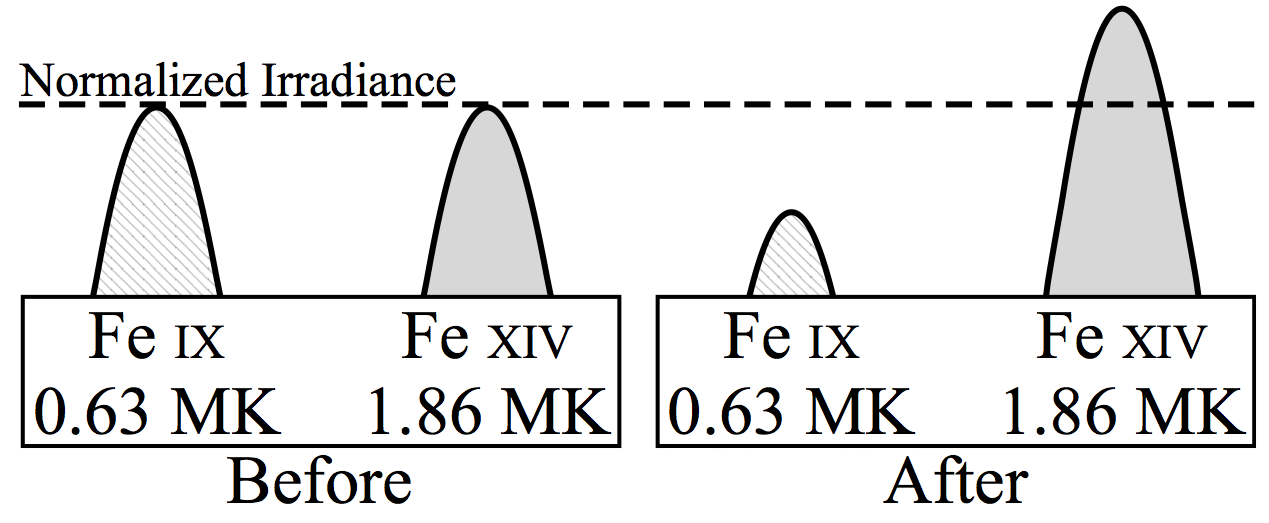
\includegraphics[width=100mm]{Images/ThermalDimming.png}
    \end{center}
    \label{thermalDimming}
\end{figure}

\section{Summary}
